\documentclass[11pt,a4paper]{article}

\usepackage[margin=1in]{geometry}
\usepackage[T1]{fontenc}
\usepackage{lmodern}
\usepackage{microtype}
\usepackage{booktabs}
\usepackage{array}
\usepackage{amsmath}
\usepackage{amssymb}
\usepackage{cite}
\usepackage{hyperref}
\usepackage{graphicx}
\usepackage{caption}
\usepackage{xcolor}
\usepackage{longtable}
\usepackage{enumitem}
\usepackage{tikz}
\usetikzlibrary{positioning,arrows.meta,shapes.geometric,calc}

\hypersetup{colorlinks=true, linkcolor=blue!50!black,
            urlcolor=blue!60!black, citecolor=blue!50!black}

% Compact tabular helper for the tables
\newcolumntype{L}[1]{>{\raggedright\arraybackslash}p{#1}}

\title{Pipeline vs.\ End-to-End Models, and Simple Ways\\
to Reduce Cascading Errors:\\
A Literature Review}

\author{Ifty Rashedul Arefin\\[2pt]
        \small Meeting~5 Report}

\date{July 9~2026}

\begin{document}

\maketitle

\begin{abstract}
This report answers two questions from Meeting~4. \emph{First:} recent
research uses ``end-to-end'' (E2E) driving models, which are one big
neural network. Our project uses a ``pipeline'' instead, which is three
separate models joined in a line: C1 (Perception, our YOLOv11n object
detector), C2 (Prediction, our constant-velocity trajectory model), and
C3 (Planning, our rule-based IDM planner). Why do we use a pipeline?
\emph{Second:}
what is a simple first method we can use to reduce cascading errors (an
error in one model spreading to the next)? I read recent papers to
answer both. The short answer to the first: in real deployed systems,
updates happen one part at a time (the perception model gets retrained
on new data, the map changes, a sensor is swapped). An E2E model is a
single block, so you cannot update just one part; you must retrain the
whole thing, which is expensive and can make the model forget what it
already knew. A pipeline lets you update the one part that changed and
leave the rest, which is how real systems are actually maintained. The
short answer to the second: build a small ``drift gate''
that checks whether a newly retrained C1 (Perception) produces very
different outputs than before, \emph{before} we let it into the pipeline.
\end{abstract}

% ============================================================================
\section{Recap of Meeting~4}
% ============================================================================
Before this literature review, a short reminder of what was done in
Meeting~4. There we ran the first real experiment on our three-part pipeline.
We trained the perception model C1 (YOLOv11n) on the Boston part of the nuScenes
data, then retrained only C1 on the Singapore part, while keeping the
prediction model C2 (constant velocity) and the planning model C3 (rule-based
IDM) unchanged. The goal was to see whether retraining a single part sends an
error down the line to the other parts (a cascading effect).

\paragraph{Experiment result.} Retraining C1 changed the downstream results
even though C2 and C3 were never touched:
\begin{itemize}[noitemsep]
    \item \textbf{C2 (prediction) got much better in the pipeline:} its error
          (minADE) dropped from $15.19$~m to $3.95$~m, about a $74\%$
          improvement, because the Singapore-tuned detector placed agents
          closer to their true positions.
    \item \textbf{C3 (planning) got slightly worse in the pipeline:} its error
          (L2 at 3~s) rose from $6.30$~m to $6.58$~m, about $+4.45\%$, even
          though C2 fed it better inputs.
    \item \textbf{The isolated (ground-truth-input) scores did not move at
          all}, which confirmed the change came only from retraining C1 and
          travelled through the pipeline, not from touching C2 or C3.
    \item \textbf{C1's own detection score (mAP) actually dropped}
          ($0.119 \to 0.064$), a small-data side effect, so the change did not
          reach C3 through the aggregate score but through the raw detections.
\end{itemize}
The interesting outcome was this mismatch: one part improving while the final
output got worse. This is the ``entangled enhancement'' pattern the project
studies, and it is the motivation for the current report, which asks why we use
a pipeline at all and how to catch such cascading effects early.

% ============================================================================
\section{Executive Summary}
% ============================================================================

\paragraph{Task~1: pipeline vs.\ E2E.} E2E models (one big network from
sensors to driving plan) are the popular trend today; one survey counts
more than 270 papers by 2024~\cite{chen2024e2esurvey}. But the same
papers admit three problems:
\begin{itemize}[noitemsep]
    \item E2E models are hard to understand and hard to
          debug~\cite{chen2024e2esurvey,hu2025vla}.
    \item You cannot fix one small part; you must retrain the whole
          model, which is slow and can make the model forget what it
          already learned~\cite{ma2025correctad,liu2025r2se}.
    \item The test score everyone reports is known to be
          unreliable~\cite{codevilla2018offline,zhai2023rethinking,dauner2023parting}.
          (This is the nuScenes \emph{open-loop} score: the model predicts
          one path for a scene, and we measure how far that path is from
          the human driver's recorded path. The car never actually drives,
          so a small distance does not prove the car would drive safely.
          We use this term throughout the report.)
\end{itemize}
This matters a lot in real deployment, where updates almost always happen
\emph{one part at a time}: a new detector is retrained on fresh data, the
map is updated, or a sensor is changed, while the other parts stay fixed.
A pipeline has three parts we can update separately, which matches this
real-world pattern. An E2E model has only one part, so every small change
means retraining everything. So a pipeline is the practical choice, not a
weaker one.

\paragraph{Task~2: reducing cascading errors.} The papers give three
groups of methods:
\begin{itemize}[noitemsep]
    \item \emph{Catch the problem early}, by checking the data passed
          between models.
    \item \emph{Retrain carefully}, so the new model does not behave too
          differently from the old one.
    \item \emph{Control the process}, by testing the new model quietly
          before using it.
\end{itemize}
We recommend one simple first method: a \textbf{drift gate} between C1
(Perception) and C2 (Prediction). Before we accept a retrained C1, we
compare its outputs to the old C1's outputs using a simple statistics
test. If they differ too much, we raise a warning.

% ============================================================================
\section{Recent End-to-End Driving Models}
% ============================================================================

An end-to-end model takes the camera and sensor input and directly
outputs the driving plan, all inside one network. Below are the most
important papers, chosen by how strong their publication is (top
conferences and journals first). The rest are listed in
Table~\ref{tab:e2e_extra}.

\paragraph{UniAD~\cite{hu2023uniad} (CVPR 2023, Best Paper).}
This is the most famous E2E model. It puts every driving task (finding
objects, tracking them, predicting their motion, and planning) into one
network, and every part is trained together to help the final plan.
\emph{Good:} it was the first ``planning-first'' unified model and won
the best paper award. \emph{Bad:} it is very heavy to train (about
144 GPU-hours) and runs slowly (1.8 frames per second)~\cite{sun2024sparsedrive};
if you want to change anything, you must retrain everything.
\emph{For us:} this is the main model we compare against.

\paragraph{VAD~\cite{jiang2023vad} (ICCV 2023).}
VAD makes E2E driving faster by describing the scene with simple lines
and vectors instead of heavy image grids. \emph{Good:} much faster than
UniAD, with similar scores. \emph{Bad:} still one big model you must
retrain all at once. \emph{For us:} together with UniAD, it is the model
that later ``repair'' papers try to fix.

\paragraph{PARA-Drive~\cite{weng2024paradrive} (CVPR 2024).}
This paper studies how to arrange the parts inside an E2E model. It shows
a design where the parts run side by side (in parallel) and can even be
turned off at run time. \emph{Good:} lower error and faster than UniAD.
\emph{Bad:} the parts still share one trained network, so you still
cannot retrain just one part. It also showed that the published
UniAD-vs-VAD comparison was not fair, because the two used different test
settings. \emph{For us:} good evidence that E2E test scores must be read
carefully.

\paragraph{SparseDrive~\cite{sun2024sparsedrive} (2024).}
SparseDrive uses a lighter scene description to make training and running
faster. \emph{Good:} it reports that it trains 7 times faster and runs
5 times faster than UniAD. \emph{Bad:} still tested only with open-loop
scores. \emph{For us:} its own numbers prove how expensive it is to
retrain a full E2E model, which supports our cost argument.

\paragraph{Hydra-MDP~\cite{li2024hydramdp} (2024, won the CVPR 2024 challenge).}
This model learns from both human driving and from a rule-based planner,
all inside one network. \emph{Good:} it won a large 2024 competition, and
it shows rule-based knowledge is still very useful. \emph{Bad:} it hides
the rule-based part inside the network, so you can no longer check or
update that part by itself. \emph{For us:} an example of why putting
everything into one block hurts maintenance.

\paragraph{Survey by Chen et al.~\cite{chen2024e2esurvey} (IEEE TPAMI 2024).}
This is the main survey of E2E driving. It lists the open problems:
E2E models are hard to understand, get confused about cause and effect,
and are not robust to new conditions. \emph{For us:} the survey is
written by E2E supporters, so when they admit these weaknesses, it is
strong evidence. Also, the survey never studies retraining policy, which
is exactly our topic. That gap is our opportunity.

\paragraph{Codevilla et al.~\cite{codevilla2018offline} (ECCV 2018).}
This early paper showed a key fact: a model's offline test score does not
always match how well it actually drives. Two models with the same score
can drive very differently. \emph{For us:} this is an honest warning we
must also apply to our own planning score.

\paragraph{Dauner et al., PDM-Closed~\cite{dauner2023parting} (CoRL 2023).}
A simple rule-based planner won the 2023 nuPlan planning challenge and
beat the learned planners. \emph{For us:} this helps in three ways:
\begin{itemize}[noitemsep]
    \item It supports our choice of a simple rule-based planner (C3).
    \item It shows that ``learned planning is better'' is not proven.
    \item It supports how we measure planning.
\end{itemize}

\paragraph{Dauner et al., NAVSIM~\cite{dauner2024navsim} (NeurIPS 2024).}
NAVSIM is a middle ground between two ways of testing. The open-loop score
(defined above) never lets the car move. The opposite is full closed-loop
simulation, where the car really drives, but that is heavy and slow.
NAVSIM sits in between: it takes the model's planned path and rolls it
forward for a short time in a light simulation, then scores useful things
like how much progress the car made and whether it would have hit
something (time to collision). These scores match real driving much better
than the open-loop distance. A large 2024 competition (143 teams) used it,
and it also found that simple models can match the big flagship models, so
extra complexity does not always help. \emph{For us:} this is the stronger
test we can move to once we need to say how well our system drives, not
just whether it got better or worse after one change.

\paragraph{Zhai et al., ``AD-MLP''~\cite{zhai2023rethinking} (2023).}
This paper showed something surprising: a tiny model using only the car's
own past motion (no camera at all) matches perception-based E2E models on
the nuScenes open-loop score. \emph{For us:} strong proof that the common
test score is weak, so we should report the collision rate too (we do)
and compare our numbers before-and-after rather than as absolute values.

\begin{table}[h!]
\centering
\caption{Other E2E and repair papers (mostly recent preprints).
These are the ``repair / maintenance'' works. They matter because they
show a new trend: even E2E research is now trying to fix models part by
part, which supports our pipeline idea.}
\label{tab:e2e_extra}
\small
\renewcommand{\arraystretch}{1.3}
\begin{tabular}{@{}L{2.4cm}L{6.7cm}L{4.0cm}@{}}
\toprule
\textbf{Paper} & \textbf{Main idea (plain words)} & \textbf{Why it matters to us} \\
\midrule
CorrectAD~\cite{ma2025correctad} (2025) &
Finds failures, makes fake training videos, then retrains the
\emph{whole} E2E model. Fixes about 62.5\% of failures. &
Proof that in an E2E model the smallest unit you can retrain is the whole
model. \\
R2SE~\cite{liu2025r2se} (2025) &
Freezes the big model and trains small add-on parts, because full
retraining makes the model forget. &
The E2E field is rediscovering modular (part-based) design. \\
ADReFT~\cite{cheng2025adreft} (2025) &
Repairs driving decisions with a separate add-on module, not by touching
the base model. &
Same lesson: add parts instead of retraining the monolith. \\
VLA survey~\cite{hu2025vla} (2025) &
Surveys the newest ``vision-language-action'' driving models. Many split
into a slow ``thinking'' part and a fast ``acting'' part. &
Even the newest models move back toward separate parts. \\
\bottomrule
\end{tabular}
\end{table}

% ============================================================================
\section{Pipeline vs.\ End-to-End: Side-by-Side}
% ============================================================================

Table~\ref{tab:e2e_vs_pipeline} compares the two designs. The last two
rows are honest: the one real strength of E2E is that it trains all parts
together. And the one real weakness of a pipeline (errors passing between
parts) is a real problem we do not hide. But note that this weakness only
appears \emph{after} an update, when one part changes and the others do
not, which is exactly the situation every deployed system faces during
maintenance. So it is a problem worth managing, not a reason to abandon
the design that real systems actually use.

\begin{table}[h!]
\centering
\caption{Pipeline (ours) vs.\ end-to-end, in simple terms.}
\label{tab:e2e_vs_pipeline}
\small
\renewcommand{\arraystretch}{1.3}
\begin{tabular}{@{}L{2.3cm}L{4.1cm}L{4.1cm}L{2.4cm}@{}}
\toprule
\textbf{Point} & \textbf{Pipeline (ours)} & \textbf{End-to-end} & \textbf{Evidence} \\
\midrule
Easy to understand & Each step (detections, predictions) can be looked at & One black box, hard to see inside & \cite{chen2024e2esurvey,hu2025vla} \\
Update one part & Can retrain any of the 3 parts alone & Must retrain the whole model & \cite{ma2025correctad,liu2025r2se} \\
Easy to debug & Can test each part alone to find the fault & Needs special methods just to locate the fault & \cite{chen2024e2esurvey,ma2025correctad} \\
Retraining cost & Retrain only the changed part (about 50~s for our C1) & Retrain everything (UniAD about 144 GPU-hours) & \cite{sun2024sparsedrive,ma2025correctad} \\
Robust to new conditions & Each part's behavior can be measured & Sensitivity and forgetting are still open problems & \cite{chen2024e2esurvey,liu2025r2se} \\
Grows easily & Add or swap parts one by one & Any change needs a new full training run & \cite{chen2024e2esurvey,sun2024sparsedrive} \\
Compute cost & Light parts run on free hardware & Slow to run, days to train & \cite{weng2024paradrive,sun2024sparsedrive} \\
Data needed & Normal labels; small fine-tunes are possible & Needs very large datasets & \cite{chen2024e2esurvey,ma2025correctad} \\
\midrule
Best overall accuracy & \emph{Weaker:} parts have different goals; some info is lost between them & \emph{Stronger:} all parts trained together & \cite{hu2023uniad,sun2024sparsedrive} \\
Trustworthy testing & Each part checked against ground truth & Common open-loop test is unreliable & \cite{codevilla2018offline,zhai2023rethinking,dauner2023parting} \\
\bottomrule
\end{tabular}
\end{table}

% ============================================================================
\section{Why We Use a Pipeline}
% ============================================================================

\paragraph{Reason 1: it matches how real systems are actually updated.}
In practice, a driving system is not retrained all at once. One part is
updated when its own data drifts (for example, the perception model is
retrained on new-city data), while the other parts stay fixed. This is
how companies actually maintain deployed systems: they fix the part that
broke, not the whole car's software. A pipeline supports this directly,
because you can update one part and leave the rest. An E2E model cannot;
its only update action is ``retrain the whole
thing''~\cite{ma2025correctad}, which means every small data change forces
a full, expensive rebuild. So the pipeline is not a smaller choice; it is
the design that matches the real update pattern of deployed systems.

\paragraph{Reason 2: a pipeline lets you find and fix faults; E2E hides them.}
The E2E side says pipelines are bad because errors pass between
parts~\cite{sun2024sparsedrive,chen2024e2esurvey}. But cascading errors do
not disappear in an E2E model; a classic industry
paper~\cite{sculley2015hidden} showed the same tangling still happens
inside one big model, it just becomes harder to see. In a real deployed
system this visibility is what matters: when something goes wrong, an
engineer must be able to point to which part failed and fix that part. A
pipeline makes that possible because each part has its own output and its
own metric. In an E2E model the fault is buried inside one network, and
the only response is to retrain everything.

\paragraph{Reason 3: real maintenance is cheaper with a pipeline.}
Deployed systems retrain again and again as the world changes: new
cities, new seasons, new sensors. With a pipeline you retrain only the
part that drifted, which for our detector takes about 50 seconds. With an
E2E model every such change forces a full retrain, about 144
GPU-hours~\cite{sun2024sparsedrive}, and repairing an E2E model can even
need generating fake failure data~\cite{ma2025correctad} because real
failure cases are rare and unsafe to collect. Over the many updates a real
system needs across its lifetime, the pipeline is far cheaper to keep
running.

\paragraph{Reason 4: even E2E research is moving back to parts.}
The clearest sign that parts matter for real use is that E2E research
itself is adding them back once maintenance becomes the goal: CorrectAD
must locate failures before fixing them~\cite{ma2025correctad}, R2SE
trains small add-on modules~\cite{liu2025r2se}, ADReFT adds a separate
repair module~\cite{cheng2025adreft}, and new VLA models split thinking
from acting~\cite{hu2025vla}. When the question changes from
``highest score on a benchmark'' to ``how do we keep this running and fix
it,'' the field moves from one block back toward separate parts, which is
exactly what a pipeline already is.

\paragraph{Reason 5: an honest note about our own testing.} The open-loop
score is weak at one job: saying ``model~A drives better than
model~B''~\cite{codevilla2018offline,zhai2023rethinking}. We do not use it
for that job. We never compare our pipeline against another model. We only
ask one question: did the planner's error go up or down after we retrained
C1, using the same planner on the same scenes? For measuring the effect of
one change on one fixed system, the score is fine. If we later want to
claim our system drives well in an absolute sense, we will switch to a
stronger test like NAVSIM~\cite{dauner2024navsim}.

\paragraph{Open problems (still unsolved by anyone).}
\begin{enumerate}[noitemsep]
    \item No paper gives a rule for \emph{which part to update, when, and
          in what order} in a real driving system~\cite{chen2024e2esurvey,hu2025vla}.
          This is a practical maintenance question every operator faces.
    \item The E2E ``repair'' area is very new (2025--2026), and its tests
          still use the weak open-loop score~\cite{ma2025correctad,liu2025r2se},
          so we do not yet know if the repairs help real driving.
    \item No one has connected software-reliability theory (availability
          and continuity, the same tools used for other safety-critical
          systems) to how these driving models are updated and maintained.
\end{enumerate}

% ============================================================================
\section{Ways to Reduce Cascading Errors}
% ============================================================================

A cascading error means: one model gets a little worse, and that makes
the next model worse, and so on down the line. Below are the strongest
papers, explained simply. The rest are in Table~\ref{tab:cascade_extra}.

\paragraph{Sculley et al.~\cite{sculley2015hidden} (NIPS 2015).}
This famous industry paper explains the core problem in one rule: in an
ML system, changing anything can change everything. When one model is
built on top of another model's output, improving one part can quietly
hurt the whole system. \emph{For us:} our E1 result (C2, Prediction, got
much better, but C3, Planning, got worse) is a clean example of exactly
this. This paper only \emph{describes} the problem; it does not give an
algorithm.

\paragraph{Data validation / TFDV~\cite{breck2019data} (SysML 2019).}
Google's method checks the data that flows between steps of a pipeline.
It compares the new data to the expected data using simple distance
measures, and raises a warning if they differ too much. \emph{Good:} used
in industry, cheap, no model change needed. \emph{Limit:} it checks the
data only, not the final score. \emph{Difficulty: easy.} This is the
model for our recommended baseline.

\paragraph{Backward-compatible training (BCT)~\cite{shen2020bct} (CVPR 2020).}
This method retrains the new model so its output still ``fits'' the old
downstream model, so you do not have to change the downstream part.
Without it, a freshly retrained model can be completely incompatible with
the old one. \emph{Limit:} keeping compatibility can slightly lower the
new model's own score, and it was designed for image search, so it needs
some adaptation for detection. \emph{Difficulty: medium.}

\paragraph{Positive-congruent training~\cite{yan2021pctraining} (CVPR 2021).}
When you update a model, some inputs that the old model got right, the new
model now gets wrong. These are called ``negative flips,'' and they
happen even when the new model is more accurate overall. This method
trains the new model to keep agreeing with the old model on those cases.
\emph{For us:} this is the same idea as our problem but at the single-example
level (better on average, worse on some cases). \emph{Difficulty: medium.}
This is our natural second method after the drift gate.

\paragraph{Ivanovic et al.~\cite{ivanovic2022propagating} (ICRA 2022).}
Normally C1 (Perception) passes only its best guess to C2 (Prediction).
This paper passes the uncertainty too, so C2 knows how sure C1 is. On a
nuScenes pipeline very close to ours, this improved prediction.
\emph{For us:} a strong ``next step'' after the baseline, but it needs
changes to how the parts talk to each other, so it is advanced.

\begin{table}[t!]
\centering
\caption{Other cascade-mitigation methods (grouped by type).}
\label{tab:cascade_extra}
\small
\renewcommand{\arraystretch}{1.3}
\begin{tabular}{@{}L{2.9cm}L{6.3cm}L{2.0cm}L{2.0cm}@{}}
\toprule
\textbf{Method} & \textbf{Main idea (plain words)} & \textbf{Type} & \textbf{Difficulty} \\
\midrule
OOD detection~\cite{nitsch2021ood} (ITSC 2021) &
Detect inputs C1 (Perception) has never seen, and trigger a safe fallback. &
Catch early & Medium \\
MOT-CUP~\cite{su2024motcup} (RA-L 2024) &
Pass C1's (Perception) uncertainty into tracking; helps most under occlusion. &
Catch early & Advanced \\
Uncertainty in planning~\cite{shao2024uncertainty} (2024) &
Planners that ignore prediction uncertainty perform worse. &
Catch early & Advanced \\
System-level view~\cite{deglurkar2024systemlevel} (2024) &
A part's quality only matters relative to the part that uses it; a
downstream part can even absorb upstream error. &
Analysis & Advanced \\
FastFill~\cite{jaeckle2023fastfill} (ICLR 2023) &
Update the model without recomputing everything downstream (which can
take months). &
Careful retrain & Medium \\
Coordinated retrain~\cite{sculley2015hidden} &
Retrain C2 (Prediction) on the new C1's (Perception) output before using
it. (Already one of our E2--E7 options.) &
Process & Easy--Med \\
Shadow / gated deploy~\cite{breck2019data} &
Run the new model quietly first; use it only if the system does not get
worse. Our isolated-vs-pipeline test is a manual version of this. &
Process & Easy \\
\bottomrule
\end{tabular}
\end{table}


\pagebreak
% ============================================================================
\section{Recommended First Baseline}
% ============================================================================

\paragraph{The idea: a drift gate between C1 (Perception) and C2 (Prediction).}
Before we accept a retrained C1 into the pipeline, we compare its outputs
to the old C1's outputs on the same fixed set of images. We look at simple
things: how many objects it finds per image, how confident it is, which
classes it predicts, and where the boxes are. We compare old vs.\ new
with two standard, simple tests. For number-type features (like the
confidence values), we use the \emph{Kolmogorov--Smirnov test}, which
measures the biggest gap between the two value distributions and gives a
single number for how far apart they are. For category-type features (like
which object classes appear), we use the \emph{Jensen--Shannon distance},
which measures how different the two category mixes are on a 0-to-1 scale
(0 means identical, 1 means completely different). This is the same idea
as \emph{Google's data validation}~\cite{breck2019data}, a widely used
industry tool that watches the data flowing between the steps of a machine
learning pipeline and raises a warning when today's data looks
statistically different from what the system expects. If the difference is
too large, we raise a ``cascade risk'' warning and do not blindly use the
new C1. Figure~\ref{fig:drift_gate} shows the idea.

\begin{figure}[h!]
\centering
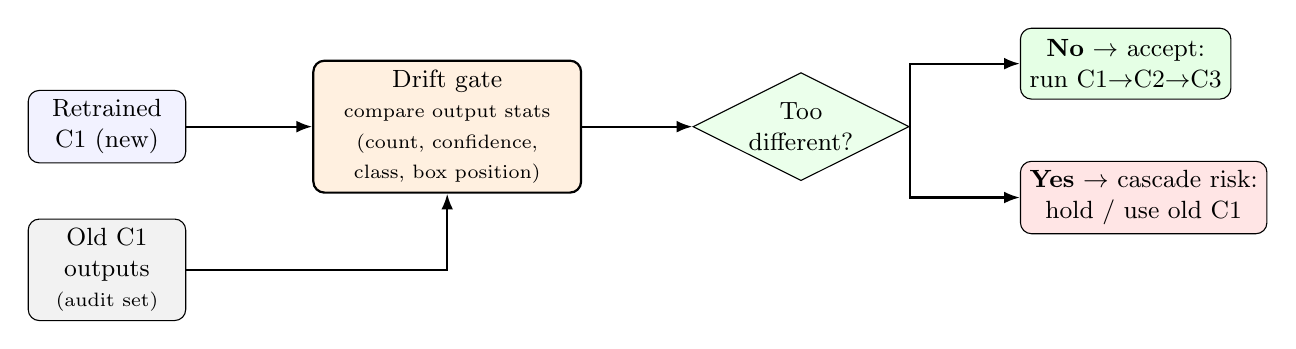
\begin{tikzpicture}[
    font=\small,
    box/.style={draw, rounded corners, minimum height=9mm, minimum width=20mm,
                align=center, fill=blue!5},
    gate/.style={draw, rounded corners, minimum height=13mm, minimum width=34mm,
                 align=center, fill=orange!12, thick},
    dec/.style={draw, diamond, aspect=2, align=center, fill=green!8, inner sep=1pt},
    pass/.style={draw, rounded corners, minimum height=9mm, align=center, fill=green!10},
    stop/.style={draw, rounded corners, minimum height=9mm, align=center, fill=red!10},
    old/.style={draw, rounded corners, minimum height=9mm, minimum width=20mm,
                align=center, fill=gray!10},
    arr/.style={-{Latex[length=2mm]}, thick},
    lbl/.style={font=\scriptsize\itshape}
]

% top row: new C1 -> gate -> decision
\node[box] (newc1) {Retrained\\C1 (new)};
\node[gate, right=16mm of newc1] (gate) {Drift gate\\\scriptsize compare output stats\\\scriptsize (count, confidence,\\\scriptsize class, box position)};
\node[old, below=7mm of newc1] (oldc1) {Old C1\\outputs\\\scriptsize(audit set)};

\node[dec, right=14mm of gate] (dec) {Too\\different?};

% outcomes
\node[pass, right=14mm of dec, yshift=8mm] (pass) {\textbf{No} $\rightarrow$ accept:\\ run C1$\to$C2$\to$C3};
\node[stop, right=14mm of dec, yshift=-9mm] (stop) {\textbf{Yes} $\rightarrow$ cascade risk:\\ hold / use old C1};

% arrows
\draw[arr] (newc1) -- (gate);
\draw[arr] (oldc1.east) -| ($(gate.south)+(0,-0.0)$);
\draw[arr] (gate) -- (dec);
\draw[arr] (dec.east) |- (pass.west);
\draw[arr] (dec.east) |- (stop.west);

\end{tikzpicture}
\caption{The drift gate. Each time C1 (Perception) is retrained, we
compare the \emph{new} C1's output statistics against the \emph{old} C1's
on a fixed set of images. If they are close, the new C1 is accepted into
the pipeline. If they differ too much, we flag a cascade risk and hold the
new C1 (or keep the old one) instead of letting the change flow silently
into C2 and C3.}
\label{fig:drift_gate}
\end{figure}

\paragraph{Why this one first.}
\begin{enumerate}[noitemsep]
    \item \textbf{Easy and free.} About 100 lines of Python over files our
          pipeline already produces. No GPU, so it fits our free Kaggle
          setup.
    \item \textbf{It would have caught our E1 case.} After the Singapore
          fine-tune, C1's (Perception) recall dropped from 0.087 to
          0.048 and its outputs clearly shifted. So we can test the gate on our
          existing v22 results right away, before running anything new.
    \item \textbf{It fits our theory.} The gate gives an early warning
          signal, which is exactly the kind of number the SMP model needs
          to estimate risk. It is also the simplest version of the
          ``entanglement forecaster'' idea from our original proposal.
    \item \textbf{It is supported by the literature.} Checking the data
          between parts is the recommended control for this
          problem~\cite{sculley2015hidden,breck2019data}, and ``better on
          average but worse on some cases'' is the exact failure it
          catches~\cite{yan2021pctraining}.
    \item \textbf{It has a clear next step.} After the gate, method B2
          (positive-congruent training) can \emph{reduce} the drift the
          gate \emph{detects}. Together they make a nice detect-then-fix
          pair for a future meeting.
\end{enumerate}

\paragraph{Honest limits.} We should be clear about what this simple gate
cannot do, so it is not oversold.
\begin{itemize}[noitemsep]
    \item \textbf{It sees change, not harm.} The gate only tells us that
          the new C1's outputs are \emph{different} from the old one's. It
          does not tell us whether that difference makes the final driving
          \emph{worse}. In fact, in our own E1 result the outputs changed a
          lot, yet C2 (Prediction) actually got \emph{better}. So a warning
          from the gate means ``look closely,'' not ``this is bad.''
    \item \textbf{The warning line has to be chosen by hand.} The gate
          fires when the difference passes a threshold, but there is no
          obvious correct value for that threshold. Set it too low and it
          cries wolf on harmless changes; set it too high and it misses
          real ones. We will have to tune it by trying values and seeing
          which ones catch the cases we care about.
    \item \textbf{We have too little data to trust the numbers yet.} With
          only 3 Singapore test scenes, we cannot yet measure how often the
          gate gives a false alarm or misses a real problem. Those rates
          need many more scenes before we can report them with confidence.
\end{itemize}
The good news is that each of these limits is itself something we can
\emph{measure} once we run the gate on real data, so this baseline is a
genuine first experiment, not just a box to tick.



\bibliographystyle{IEEEtran}
\bibliography{references}

\end{document}
